\documentclass[11pt]{article}
\usepackage{deauthor,times,graphicx}
\usepackage{subfig}
\graphicspath{{submissions/teach-qp-bhowmick/figs/}}

\usepackage{balance}
\usepackage{xspace}
\usepackage{url}
\usepackage{hyperref}
\usepackage{authblk}
\usepackage{cite}

\newcommand{\ie}{\emph{i.e.,}\xspace}
\newcommand{\eg}{\emph{e.g.,}\xspace}
\newcommand{\etc}{\emph{etc.}\xspace}
\newcommand{\wrt}{\emph{w.r.t.}\xspace}
\newcommand{\resp}{\emph{resp.,}\xspace}
\newcommand{\etal}{\emph{et al.}\xspace}
\newcommand{\btitle}[1]{\vspace{1ex}\noindent \textbf{#1}}
\newcommand{\eat}[1]{}
\def\EndOfProof{\nolinebreak\ \hfill\rule{1.5mm}{2.7mm}}

\begin{document}
\title{Towards Technology-Enabled Learning of Relational Query Processing}
\author{Sourav S.\ Bhowmick$\,^{\star}$~~~and~~~Hui Li$\,^{\diamond}$\\ $^{\star}$~Nanyang Technological University (NTU), Singapore, \texttt{assourav@ntu.edu.sg}\\
$^{\diamond}$~Xidian University, China, \texttt{hli@xidian.edu.cn}
}
\maketitle

\begin{abstract}
The database systems course has gained increasing prominence in academic institutions due to the convergence of widespread usage of relational database management system (\textsc{rdbms}) in the commercial world, the growth of Data Science, and the increasing importance of lifelong learning. A key learning goal of learners taking such a course is to learn how \textsc{sql} queries are processed in an \textsc{rdbms} in \emph{practice}. Most database courses supplement traditional modes of teaching with technologies such as off-the-shelf \textsc{rdbms} to provide hands-on opportunities to learn database concepts used in practice. Unfortunately, these systems are not designed for effective and efficient pedagogical support for the topic of relational query processing. In this vision paper, we identify novel problems and challenges that need to be addressed in order to provide effective and efficient technological supports for learning this topic. We also identify opportunities for \textit{data-driven} education brought by any effective solutions to these problems. Lastly, we briefly report the \textsc{truss} system that we are currently building to address these challenges.
\end{abstract}


%====================================================================================================
\section{Introduction}  %17
\label{sec1}
%====================================================================================================
Learning is the acquisition of knowledge or skills through study, experience, or being taught~\cite{Gross}.  It is not just listening and accepting what we are taught, but understanding and experiencing them. Education, on the other hand, is the acquisition of knowledge through a process of receiving or giving systematic instruction. Hence, although learning and education are closely related, the former has a broader scope and impact. Specifically, learning can be facilitated through education, personal development, schooling, training or experience. It is not limited to a certain age or period in life. Indeed, while formal education for young adult learners at universities has been the focus of educational provisions in the industrial age, the digital age is now seeing an increased experimentation of  ``lifelong learning''~\cite{unesco} with provisions such as  work-study programmes for early career and mid-career individuals, and digital learning initiatives.

The growing demand for lifelong learning coupled with the widespread use of relational database management system (\textsc{rdbms}) in the commercial world and the growth of Data Science as a discipline have generated increasing demand of database-related courses in academic institutions. Learners from diverse fields and experiences aspire to take these courses, even with limited Computer Science backgrounds~\cite{panel}. In a computer science degree program, the key goal of a database systems course is to teach learners how to \emph{build} a database system. On the other hand, the focus of the course in a data science program is to be able to \emph{control} a database system effectively. To facilitate both these goals, it is paramount for learners to learn  how \textsc{sql} queries are processed in an \textsc{rdbms} in practice. Traditionally, this learning goal is achieved through textbooks and lectures. Specifically, major database textbooks~\cite{dbtext,cow} introduce \textit{general} (\ie not tied to any specific \textsc{rdbms}) theories and principles associated with relational query processing and optimization using natural language-based narratives and visual examples. This allows a learner to gain a general understanding of \textsc{sql} query execution strategies. 

It is well-established in education that \textit{effective} use of technology has a positive impact on learning~\cite{HXK12}. It causes learners to be more motivated and engaged, thus, enabling them to retain more information. It also increases hands-on learning opportunities. In fact, technology is best used as \textit{``a supplement to normal teaching rather than as a replacement for it''}~\cite{HXK12}. Hence, in order to promote effective and efficient learning for diverse individuals in full recognition of the complexity of the topic of relational query processing,  \emph{learner-friendly} tools are paramount to  augment the traditional modes of learning (\ie textbook, lecture).  Indeed, database systems courses in major institutions around the world supplement traditional style of learning with the usage of off-the-shelf \textsc{rdbms}. Unfortunately, these \textsc{rdbms} are not designed for pedagogical support. Although they enable hands-on learning opportunities to build database applications and pose a wide variety of \textsc{sql} queries over it, very limited effective and efficient learner-friendly support, beyond the visualization of \textit{query execution plans}, is provided for understanding and experiencing the processing and optimization of these queries \textit{in practice} by the underlying relational query engine. 


Given the challenges faced by learners to learn \textsc{sql}~\cite{MAF21}, there has been increasing research efforts to build tools and techniques to facilitate comprehension of complex \textsc{sql} statements~\cite{KV+12,HM+22,MRY19,MF21,LZ+20,DG11}, automated grading of \textsc{sql} queries~\cite{BC+15}, and so on. However, scant attention has been paid to explore technologies that can enable learning of relational query processing~\cite{lantern,neuron,picasso}. In this paper, we articulate a vision shaped by the following fundamental questions: (a) What are the key problems that we need to address to facilitate technology-enabled learning of relational query processing in practice? (b) How can the potential solutions to these problems support data-driven education with the goal of making teaching and learning practices more effective and efficient?  Specifically, our vision calls for a \textit{learning-centric}, \textit{generic}, and \textit{psychology-aware} approach grounded on the \textit{theories} of motivation and learning to address these challenges. Note that by no means we claim that the list of problems discussed in this article is exhaustive. The pervasive desire here is to galvanize the data management community to explore this nascent inter-disciplinary topic at the intersection of learning sciences and data management by leveraging these problems as the seed.

The rest of the paper is organized as follows. In Section~\ref{back}, we briefly introduce relevant \textit{motivation theories} that are at the foundation of learning and may potentially impact the design of any learner-centric, technology-enabled solutions for learning. Section~\ref{sec:challenge} introduces the  key novel research challenges that need to be addressed in order to realize the vision. We briefly report the \textsc{truss} system which we are currently building to address these challenges in Section~\ref{sec:truss}. The last section concludes this paper.
  
%====================================================================================================
\section{Motivation Theories}
\label{back} 
%====================================================================================================

Learning is impacted by \textit{motivation}, which is the process that initiates, guides, and maintains goal-oriented behavior~\cite{kazdin}. Specifically, motivation impacts how likely a learner is willing to learn. Since effective use of technology in learning has positive impact on motivation,  we need to understand motivation theories and their impact on learning. These theories should underpin any effective technological solutions for facilitating learning. In this section, we first briefly describe key theories related to motivation proposed in the domain of education psychology. Next, we highlight how these theories can guide technology-enabled solutions for learning. In the next section, we shall identify novel research issues that are grounded on these theories to facilitate learning of relational query processing.

\vspace{1ex} \noindent \textbf{Motivation theories.} Motivation can be broadly characterised into two types,\textit{ intrinsic} and \textit{extrinsic}~\cite{RD00}.\textit{ Intrinsic motivation} is the act of doing an activity purely for the joy of doing it whereas \textit{extrinsic motivation} is to do something due to the influence of external  rewards or punishments (\eg good grades, jobs). Although the latter is not optimal for learning, research suggests that extrinsic motivation is prevalent~\cite{RD00,DV+91} and may pave the way to intrinsic motivation. That is, a learner may initiate learning due to external factors but the motivation may morph to an intrinsic one during task engagement. 
 
Regardless of the type of motivation, \textit{Achievement Goal Theory}~\cite{AP12} argues that all motivation are essentially linked to one's goals that can take two forms, namely \textit{performance goals} and \textit{mastery goals}. The former is caused by satisfaction of one's ego (\eg appearing superior to one's peers) whereas the latter is aligned with intrinsic motivation and is grounded on the pure desire to master a skill or concept. The \textit{Expectancy Value Theory}~\cite{WE00} postulates that expectation and value of learning a skill or concept have direct impact on the performance and task choice of a learner. To elaborate further,  an individual's effort and performance for a task are influenced by their expectation of success or failure.  Note that expectations and values themselves are influenced by how a learner assess their competency and perceived task difficulty.  If a learner has felt satisfaction in undertaking a similar task in the past, then it is more likely they will put effort to the current task.  However, if past experience shows the task is either too difficult to be completed or not sufficiently difficult enough then they may not engage with it. The \textit{Flow Theory}~\cite{NL09} describes a  psychological state in which an individual is purely intrinsically motivated to learn without any external factors. Such state is said to occur when the task is neither too difficult to cause helplessness or frustration nor too easy to make a learner bored. 

\vspace{1ex} \noindent\textbf{Motivation theories in technology-enabled learning frameworks.} Every learner has intrinsic or extrinsic motivation to reach their learning goals. Hence, any technology-enabled learning framework should be cognizant of the above theories in order to cultivate motivation to learn. Specifically, technologies to supplement learning of relational query processing and optimization should support the followings:

\begin{itemize} \itemsep = -0.5ex

\item Learners may learn relational query processing due to intrinsic or extrinsic motivation. It is important that any technological framework support both and facilitate transformation of extrinsic motivation to intrinsic one during the course of interacting with it. 

\item  Increase learners' satisfaction of successful completion of the task of learning relational query processing as well as facilitate flow state of learners to move to the Goldilock's zone (\ie learning relational query processing concepts is neither too difficult nor too easy). 

\end{itemize}

%====================================================================================================
\section{Research Issues}
\label{sec:challenge}
%====================================================================================================
In this section, we outline novel \textit{learner-centric} research issues in the burgeoning topic of technology-enabled learning of relational query processing.  It is worth noting that although technology engages and motivates learners, it is advantageous for learning only when it is aligned to with what is to be learned~\cite{HXK12}. Hence, the issues we focus for technological support are learning about query execution plans, exploration of \textit{alternative query plans} in a plan space, and cost estimation of a physical query plan. Observe that all these issues are typically covered by a database systems course.  A common theme that cuts across these issues is the pervasive desire for motivation theory-aware tools and techniques that aim to \emph{supplement} existing off-the-shelf \textsc{rdbms} to facilitate learning of these issues. We begin with a brief background on relational query plans that learners typically encounter in a database systems course. 

%====================================================================================================
\subsection{Query Plans}
%====================================================================================================

Given an arbitrary \textsc{sql} query, an \textsc{rdbms} generates a \textit{query execution plan} (\textsc{qep}) to execute it.  A \textsc{qep}  consists of a collection of physical operators organized in form of a tree, namely the \textit{physical operator tree} (\textit{operator tree} for brevity). Figure~\ref{fig:alter_plans}(a) depicts an example \textsc{qep} with a collection of physical operators. Each physical operator, \eg \texttt{SEQUENTIAL SCAN}, \texttt{INDEX SCAN}, takes as input one or more data streams and produces an output one. A \textsc{qep} explicitly describes how the underlying \textsc{rdbms} shall execute the given query. Notably, given an \textsc{sql} query, there are many different query plans, other than the \textsc{qep}, for executing it.  We refer to these different plans (other than the \textsc{qep}) as \textit{alternative query plans} (\textsc{aqp}).  Figures~\ref{fig:alter_plans}(b)-(c) depict two examples of \textsc{aqp}. 
 
 
 \begin{figure}[t]
	\centering
	\includegraphics[width=0.95\linewidth]{motieg.pdf}
	\vspace{0ex}\caption{Examples of \textsc{qep} and alternative query plans.}
	\label{fig:alter_plans}
	%\hrule
	\vspace{0ex} \end{figure}

%====================================================================================================
\subsection{Understanding Query Execution Plans (QEPs)} \label{sec:nlg}
%====================================================================================================
A key goal of learning relational query processing is to understand  how \textsc{sql} queries are processed in an \textsc{rdbms} in practice. This can be achieved by understanding the content of the \textsc{qep} of a given query.  Major database textbooks (\eg \cite{dbtext,cow})  typically illustrate \textsc{qep}s of simple \textsc{sql} queries, their costs, and  adverse impact on estimated cost if alternative physical operators are chosen (\eg merge join instead of hash join) for a \textsc{qep}. However, they are not interactive and the variety of examples they can discuss is constraint by the page limit and cost. Hence, only a very few simple, static examples of \textsc{qep}s are typically exposed to learners.

Off-the-shelf \textsc{rdbms} (\eg PostgreSQL) provide the opportunity to greatly mitigate the limitations of textbooks. A learner may implement a database application in an \textsc{rdbms}, pose queries over it, and peruse the associated \textsc{qep}s to comprehend how they are processed by an industrial-strength query engine in practice. Such interactivity provides learners the freedom to formulate a large number of queries with diverse complexities and view the contents of corresponding \textsc{qep}s in real-time. 

Most existing \textsc{rdbms} expose the \textsc{qep} of an \textsc{sql} query using \textit{visual} or \textit{textual} (\eg unstructured text, \textsc{json}, \textsc{xml}) format.  Unfortunately, comprehending these semistructured textual formats to learn about query execution strategies of \textsc{sql} queries in practice can be daunting for learners. In contrast to natural language-based narrations in database textbooks, they are not user-friendly and assume deep knowledge of vendor-specific implementation details.  On the other hand, the visual format is relatively more user-friendly but hides important details. Consequently, in consistent with the \textit{Expectancy-Value Theory}, the task difficulty may become a barrier for some learners to learn about query execution strategies in a specific \textsc{rdbms} from these \textsc{qep} formats.  

\begin{example} \label{eg:1}
Doreen is an undergraduate student in a data science program who is currently enrolled in a database course. She wishes to understand the execution steps of the following \textsc{sql} query in PostgreSQL on the IMDb benchmark dataset~\cite{imdb} by perusing the corresponding \textsc{qep} in Figure~\ref{fig:plan}(a) (partial view). 
\begin{quote}
\begin{verbatim}
SELECT mc.note AS production_note, 
	   t.title AS movie_title, 
	   t.production_year AS movie_year
FROM company_type AS ct, 
	 movie_companies AS mc, 
	 movie_info_idx AS mi_idx, 
	 title AS t
WHERE ct.kind = 'production companies'
	  and mc.note like '%(co-production)%'
	  AND ct.id = mc.company_type_id
	  AND t.id = mc.movie_id 
      AND mc.movie_id = mi_idx.movie_id;
\end{verbatim}
\end{quote}
 Unfortunately, Doreen finds it difficult to mentally construct a narrative of the overall execution steps by simply perusing it. This problem is further aggravated in more complex \textsc{sql} queries. Hence, she switches to the visual tree representation of the \textsc{qep} as shown in Figure~\ref{fig:plan}(b). Although relatively succinct, it simply depicts the sequence of operators used for processing the query, hiding additional details about the query execution (\eg sequential scan, join conditions).  In fact, Doreen needs to manually delve into details associated with each node in the tree for further information.
\EndOfProof
\end{example}

Since natural language (\textsc{nl})-based narratives aided with visual examples (as in textbooks and lectures) have been the traditional mode of learning for decades, we advocate that an  intuitive natural language (\textsc{nl})-based description of a \textsc{qep} can greatly augment learning of the execution strategies of \textsc{sql} queries by an \textsc{rdbms}. The intuition is that \textsc{nl}-based descriptions may facilitate the flow state of learners (\textit{Flow Theory}) to the Goldilock's zone. This can then effectively complement the current visual tree format generated by existing  \textsc{rdbms}.  Specifically, a learner may either use the visual \textsc{qep} to get a quick overview and then peruse the \textsc{nl} description or study them in parallel to acquire detailed understanding. To support this hypothesis, we surveyed 62 and 56 unpaid volunteers taking the undergraduate database course in NTU in two semesters (2019 and 2020).  We use the \textsc{tpc-h} v2.17.3 benchmark  and a  rule-based natural language generation tool for \textsc{qep}s ~\cite{neuron} to generate natural language descriptions of \textsc{qep}s for \textsc{sql} queries formulated by the volunteers.  The volunteers were asked: \textit{``which query plan format they prefer for learning?''} 53.2\% and 55.4\% preferred \textsc{nl}-based description, respectively. Very few (3\% and 5.4\%, respectively) preferred the text format. Hence, there is clear evidence that learners prefer to use \textsc{nl}-based and visual tree-based formats for learning about \textsc{qep}.

\begin{figure}[t]
\centering
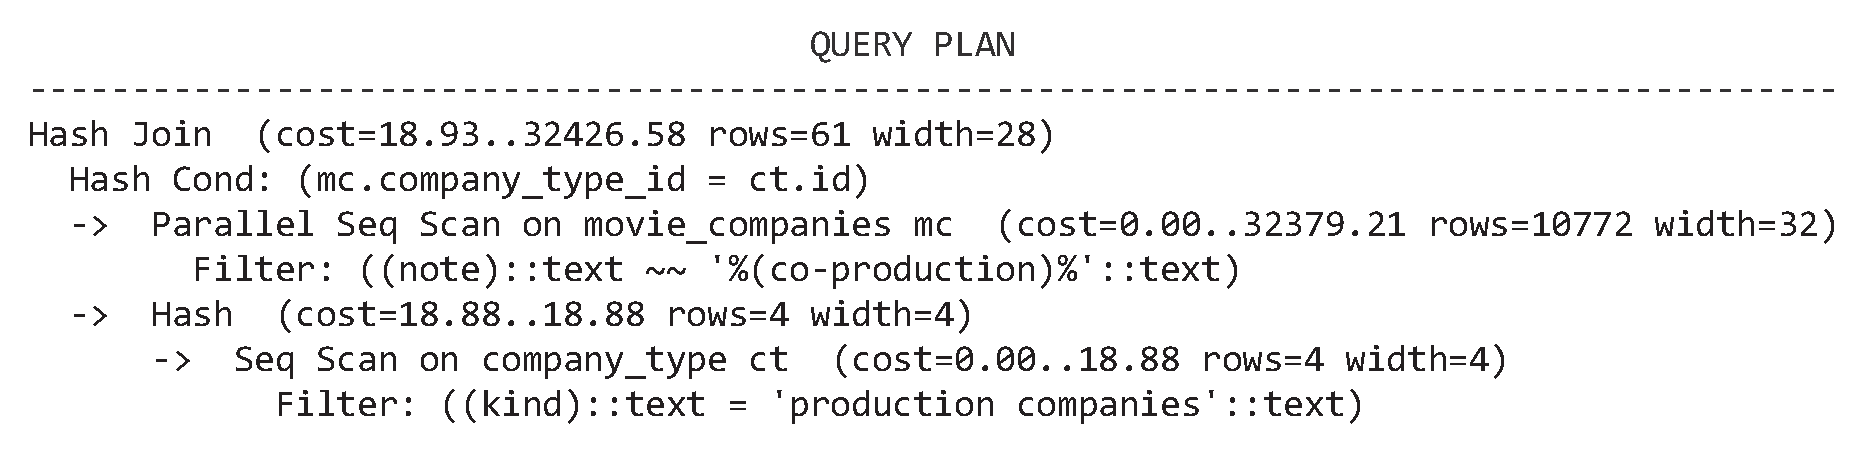
\includegraphics[width=0.45\linewidth]{newfig1.eps}
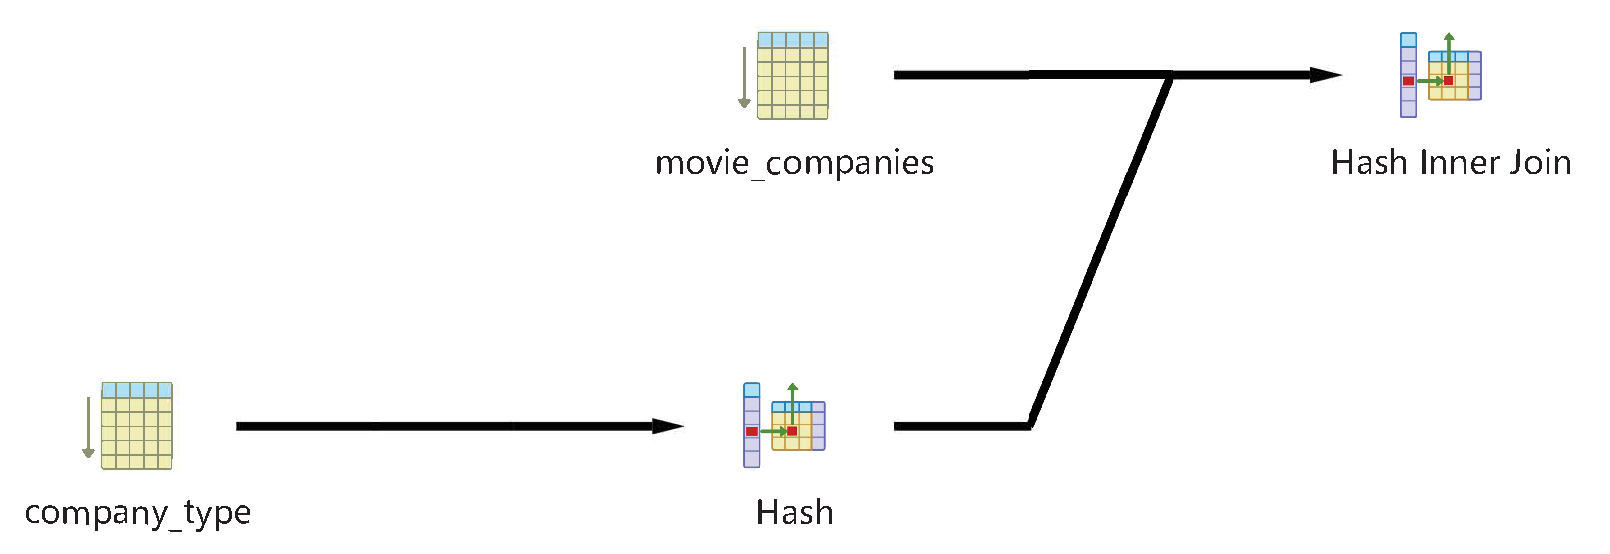
\includegraphics[width=0.5\linewidth]{sdf.eps}
\vspace{0ex}\caption{A \textsc{qep} in PostgreSQL and its visual tree representation.}
\label{fig:plan}
%\hrule
\vspace{0ex}\end{figure}


The majority of \textsc{nl} interfaces for \textsc{rdbms}~\cite{KS+20}, however, have focused either on translating natural language sentences to \textsc{sql} queries or narrating \textsc{sql} queries in a natural language. Scant attention has been paid for generating natural language descriptions of \textsc{qep}s~\cite{neuron,lantern}, which is a challenging problem.
Although deep learning techniques, which can learn task-specific representation of input data, are particularly effective for natural language processing, it has a major upfront cost. These techniques need massive training sets  of labeled examples to learn from. Such training sets in our context are prohibitively expensive to create as they demand database experts to translate thousands of \textsc{qep}s of a wide variety of \textsc{sql} queries.  Even  labeling using crowdsourcing is challenging as accurate natural language descriptions demand experts who understand \textsc{qep}s. Note that accuracy is critical here as low quality translation may adversely impact individuals' learning.

%====================================================================================================
\subsection{Learning Impact of Alternative Choices on QEP} \label{sec:impact}
%====================================================================================================
Natural language description of a \textsc{qep} enables a learner to understand the execution steps of a query. This may pique the interest of a learner to raise further questions related to query processing centred around a specific \textsc{qep}. Since major database textbooks typically discuss the adverse impact of choosing alternative physical operators or join ordering on the estimated cost, a learner may also like to delve deeper into the impact of these alternative choices on the estimated query processing cost of their queries.

\eat{This may be due to the shift from extrinsic motivation to intrinsic one to learn about relational query processing.}

\begin{example}  \label{eg:2} 
Reconsider Example~\ref{eg:1}. Doreen's course lectures and textbook discuss the impact of physical operator choices and join ordering  on the selection of a \textsc{qep}. Hence, after perusing the content of the \textsc{qep},  she wonders what will be the impact on the cost be if the hash join is replaced by a merge join? Is the estimated cost of the alternative query plan substantially higher compared to the \textsc{qep}? How much is the impact on the estimated cost if the join ordering is changed?   In this context, a narrative that explains why the \textsc{qep} is chosen by connecting its content with knowledge garnered from database textbooks will greatly benefit her learning. 
\EndOfProof
\end{example}

Unfortunately, as stated earlier, off-the-shelf \textsc{rdbms} are not developed for pedagogical support.  Typically, they do not expose the impact of alternative choices of various physical operators or join ordering on the \textsc{qep} in a \emph{user-friendly} manner to aid learning.  Note that such information is invaluable to learners as it not only facilitates hands-on inquire-driven learning on the impact of a choice of a physical operator  or a specific join ordering on the estimated cost of a \textsc{qep} but it also enables them to comprehend why a \textsc{qep} is chosen by the underlying \textsc{rdbms}. However,  an \textsc{rdbms} typically demands a learner to manually pose \textsc{sql} queries with various constraints on \textit{configuration parameters} (\textit{e.g.}, \texttt{enable\_hashjoin}, \texttt{enable\_nestloop} in PostgreSQL) to view the corresponding \textsc{qep} containing specific physical operators. Furthermore, one has to manually compare the generated plan with the original \textsc{qep} to understand the impact. Notably, a database course may not introduce these configuration parameters while exposing syntax and semantics of \textsc{sql}. It is also impractical to assume that learners will be familiar with them  when many are taking the course for the first time.  Clearly, based on the \textit{Expectancy-Value} and \textit{Flow} theories, a learner-friendly framework that can facilitate exploration of the impact of various physical operators and join ordering on a \textsc{qep} can greatly motivate learners to deeper engagement and learning of this topic. 

Intuitively,  given  an \textsc{sql} query and learner-specified \textit{preferences} (\eg merge join, index scan, specific join ordering), the goal is to automatically visualize the impact of these choices on the selected \textsc{qep}. In this context, it is important to generate a natural language-based explanation that goes beyond the conventional least-cost-based explanation to connect established knowledge related to usage scenarios of different physical operators from textbooks with the specified preferences. For instance, examples of some established knowledge are:  (a) index scan is the optimal access path for low selectivity whereas sequential scans perform better in high selectivity~\cite{borovicaGajic2018}; (b) merge join is preferred if the join inputs are large and are sorted on their join column~\cite{msdn}; (c) nested-loop join is ideal when one join input is small (\eg fewer than 10 rows) and the other join input is large and indexed on its join columns~\cite{msdn}. Such knowledge in the form of explanations will naturally facilitate learners' understanding of relational query processing. For instance, consider Example~\ref{eg:2}. Explanations such as (b) will help Doreen to understand why a hash join was chosen by the relational query engine.

The problem is challenging from several fronts. While under-the-hood it is straightforward to generate an \textsc{sql} query involving the learner-specified preferences and retrieve the corresponding \textsc{qep}, automatically generating appropriate visualization framework to aid learning is challenging. First, how should the results be presented in consistent with motivation theories to motivate learners to explore and learn? Note that a learner may want to view the impact of multiple physical operators and join ordering together instead of just a single operator or join ordering. Simply generating an \textsc{nl} description of the \textsc{aqp} is insufficient since this will demand a learner to manually compare the description of the original \textsc{qep} with it in order to understand the impact of various operators and join ordering. Naturally, this becomes tedious especially for complex queries.  Second, how can we generate  \textsc{nl} explanations that augment learning by connecting with textbook knowledge? It demands sophisticated text extraction, analytics, and summarization framework that connects the alternative query plans with relevant established knowledge embedded in online resources.   

%====================================================================================================
\subsection{Exploration of Informative Alternative Query Plans} 
%====================================================================================================
In the preceding challenge, a learner has clear preferences that they wish to explore with respect to a \textsc{qep}. However, this may not always be the case.  Some learners may not have clear idea of what alternative query plans they are interested in.\eat{ Consider the following example scenario.} 

\begin{example}\label{eg:3}
 Meng is another undergraduate student pursuing a degree in computer science and a classmate of Doreen in the database course. He also formulates the query in Example~\ref{eg:1}. After viewing the \textsc{qep}, he wonders what are the different alternative query plans (\textsc{aqp}s) considered by the underlying \textsc{rdbms} during the \textsc{qep} selection process. Specifically, are there alternative plan(s) that have similar (resp. different) structure and physical operators but very different (resp. similar) estimated cost? If there are, then how they look like? 
\EndOfProof
\end{example}


Off-the-shelf \textsc{rdbms} do not expose a \textit{representative} set of alternative query plans considered by the underlying query optimizer during the selection of a \textsc{qep} in a \emph{user-friendly} manner to aid learning. Hence, due to the lack of easy access to such information in \textsc{rdbms}, based on the \textit{Expectancy-Value Theory}, learners may restrict themselves to the simple and limited number of examples that are typically exposed in textbooks and lectures or simply abandon the effort. Clearly, a learner-friendly framework that can facilitate retrieval and exploration of ``informative'' alternative query plans associated with a given query can greatly aid in answering Meng's questions related to the query optimization process. 

Selecting a set of \textit{informative} \textsc{aqp}s to facilitate learning is a technically challenging problem. First, what is an ``informative'' \textsc{aqp} in the context of learning? To elaborate further, reconsider Example~\ref{eg:3}. Figures~\ref{fig:alter_plans}(b)-(c) depict two alternative plans for the query where the physical operator/join order differences are highlighted with red rectangles and significant cost differences are shown using yellow nodes. Specifically, \textit{AP1} has very similar structure as the \textsc{qep} but different join order involving \texttt{title} and \texttt{company\_type} relations and significantly different estimated cost. \textit{AP2}, on the other hand, displays similar estimated cost as the \textsc{qep}  but different join order. \textit{Which of these alternative plans should be revealed to Meng?} The overarching goal here is to  choose alternative plan(s)  that may enhance Meng's knowledge of the \textsc{qep} selection process (\ie informative) as well as motivate him to learn and explore. Certainly, any \textit{informativeness} measure needs to be cognizant of plans that a learner have already viewed for her query (including the \textsc{qep}) in order to avoid the exposure of highly similar information. It should also facilitate retrieval of plans that learners may be interested in as far as query optimization is concerned. Hence, it is paramount to take feedback from learners on the \textit{types} of \textsc{aqp}s that are potentially of interest to them and devise a mechanism to quantify \textit{informativeness} of a plan by mapping the knowledge acquired from the feedback to a \textit{utility} measure. Subsequently, we need to design techniques that can select informative plans that  \textit{maximize} the \textit{utility} as we cannot simply rely only on the estimated cost of alternative plans.  Second, the number of candidate \textsc{aqp}s for a given \textsc{sql} query is exponential in the worst case~\cite{SC98}. Hence, it is prohibitively expensive to scan all these plans to select informative ones. Note that the selection of \textsc{aqp} cannot be integrated into the plan enumeration step of the underlying query optimizer. We need to know the \textsc{qep} when computing \textsc{aqp} as they are selected with respect to the \textsc{qep} a learner has seen. 
	
At first glance, it may seem that we can select $k>1$ alternative query plans where $k$ is a value specified by a learner. Although this is a realistic assumption for many top-$k$ problems, learners may not necessarily be confident to specify the value of $k$ always. They may prefer to \textit{iteratively} view one plan-at-a-time and only cease exploration once they are satisfied with the understanding of the query optimization process for a specific query. Hence, $k$ may not only be unknown \textit{apriori} but also the selection of an \textsc{aqp} at each iteration to enhance learning of different plan choices depends on the plans viewed by a learner thus far. Clearly, it does not increase learners' understanding of the query optimization process or motivate them to use the framework if a plan with highly similar information of an already viewed plan is revealed to them in the subsequent iterations. This demands for a flexible solution framework that can select informative \textsc{aqp}s in absence or presence of the $k$ value. 


%====================================================================================================
\subsection{Understanding Cost Estimation of a Physical Query Plan}  \label{sec:cost}
%====================================================================================================
The preceding subsections introduce research issues that aim to facilitate learning of the execution strategy of an \textsc{sql} query and  interesting plan choices a relational query optimizer makes in practice. Another key knowledge that a learner needs to acquire is the cost estimation procedure of these plans.   

\begin{example}\label{eg:4}
 Doreen and Meng have learnt from textbooks and lectures how the cost of a physical query plan can be estimated. However, the number of queries considered in these modes of learning and their complexities are limited. They are motivated to experience cost estimation of plans associated with a wider variety of queries. Hence, they pose several queries with different degrees of complexity on the IMDb dataset in PostgreSQL. They can view the overall estimated cost of a \textsc{qep} as well as cost of different subtrees (\eg Figure~\ref{fig:alter_plans}). However, they cannot view step-by-step details of the input parameters and the formulas used by the underlying query optimizer to compute these numbers. For instance, in Figure~\ref{fig:alter_plans}(a), why is the cost of the first \texttt{HASH JOIN} \textit{2046.6}? By undertaking a back-of-the-envelope calculation using formulas learnt in the course, they could not replicate this value. Are some of the principles and formulas to compute cost different from what they have learnt from textbooks and lectures? If so, then why? 
 
 Doreen and Meng also wonder what the intermediate result sizes of different operations are here? When they execute one of the queries, they have to wait for a considerable amount of time to view the results. Does the estimated time cost of the \textsc{qep} differ significantly from the actual cost? Why? 
\EndOfProof
\end{example}

Existing \textsc{rdbms} do not provide any learner-friendly support to facilitate such learning. Consequently, based on motivation theories, learners may not pursue this direction of inquiry using an \textsc{rdbms}, surrendering valuable opportunity for hands-on acquisition of knowledge of the cost estimation process. It is challenging, however, to expose an interface to facilitate such learning and exploration. First, it demands automated analysis of the code base of the underlying query optimizer to extract various formulas used for cost estimation. These formulas may not necessarily be identical across all \textsc{rdbms} or textbooks. For instance, in~\cite{dbtext}, the cost of a selection involving inequality condition is approximated to be 1/3 of the input size independent of the selection condition. On the other hand, in~\cite{cow}, more accurate measure is used for estimating the selection cost.  Furthermore, a specific \textsc{rdbms} may implement variants of these formulas. Second, it is paramount to connect these formulas with specific input parameters for a query to reveal how the cost of a plan is estimated while emphasizing the similarity and differences with textbook knowledge. A framework that can support this in a palatable manner to facilitate learning is non-trivial as it may demand a sophisticated natural language generation framework that connects analysis of the code base with textbook content. Third, superior visualization and \textsc{nl}-based framework are necessary to explain to learners the reasons for the differences in estimated and actual cost of a query. Although tools such as~\cite{picasso} allow one to visualize the cost of different plans over the plan space,  they are not designed for explaining the \emph{cost differences} for a \emph{specific} query in a palatable manner. 

%====================================================================================================
\subsection{A Unifying Framework: Chatting with a Relational Query Engine} 
%====================================================================================================

\begin{figure}[t]
\centering
\includegraphics[width=\linewidth]{chatbot.pdf}
\vspace{0ex}\caption{An example of interaction between a learner and the chatbot.}
\label{fig:chatbot}
%\hrule
\vspace{0ex}\end{figure}

Although addressing the aforementioned issues has the potential to facilitate learning of relational query processing by providing learner-friendly platforms, a set of isolated platforms that address these different issues will make it cumbersome for learners to navigate and take advantage of them.  For instance, learners may find it overwhelming to operate three independent technology-enabled learning platforms targeting \textsc{nl} description generation of \textsc{qep}, exploration of \textsc{aqp}, and cost analysis of query plans, respectively. This may deter them to use such technology for learning. Given that young adults often interact through chat apps (\eg Whatsapp, WeChat), a natural language interaction framework (\ie chatbot) that can unify these solutions may bring practical benefits to learners.  A possible interaction between a learner and a hypothetical chatbot designed for interacting with a relational query engine are shown in Figure~\ref{fig:chatbot}.

Building a high-quality chatbot for a relational query engine to facilitate learning is non-trivial and challenging.  In addition to the challenges mentioned earlier for addressing individual components, a chatbot brings new challenges with respect to correct parsing and interpretation of a learner's statement, constructing correct (syntactically and semantically) responses in a natural language, engaging learners in conversations, and so on. While these challenges are long recognized in building a generic chatbot~\cite{GGL18}, the domain-specific nature of the problem brings in interesting flavor to it. Different from natural conversations, a learner’s questions usually have concrete objectives, actively requesting information, and an answer to every question should facilitate understanding of relational query processing. Furthermore, a learner's questions at each step are not only closely related to the chatbot’s current answers, but also need to take into account the context of the previous parts of the conversation. For example, consider the first three questions in Figure~\ref{fig:chatbot} from the learner. These questions are actively requesting information related to relational query processing. Observe that the third question is related to the preceding parts of the conversation.  

Any chatbot needs to consider two kinds of information in a learner's question: (1) the intent of the question (\eg understanding cost computation) and (2) the content of the question (\eg cost computation steps of zigzag join in a \textsc{qep}).  To this end, we can construct a \textit{query processing knowledge graph} semi-automatically to represent a collection of relational query processing concepts. Then the intent and content can be determined by \textit{mapping} the question to different concepts in the knowledge graph. Note that similar idea of knowledge graph has been recently exploited in the context of question generation for multi-party court debates for judicial education~\cite{ZJ+22}. Once the intent and content of a question are determined, the chatbot invokes the relevant component (Section~\ref{sec:nlg}-\ref{sec:cost}) to retrieve the answer for the specific question. The result returned by it is then \textit{transformed} into a natural language (supported by visual representations, if necessary) and presented to the learner.

   

  \begin{table*}[t]
\centering
 \caption{\label{tab:learn}Learning-centric issues.}
 \scriptsize
 \begin{tabular}{|p{70mm}|p{77mm}|}
  \hline
  \textbf{Issue} & \textbf{Questions to address}  \\
  \hline
 \textbf{ \textit{Rational for the impact of technologies on learning}} & Will learners work more efficiently, more effectively, more intensely? \\
 & Will the technology help them to learn for longer, more deeply, more productively? \\ \hline
\textbf{\textit{Role of technology in learning}} & Will it help learners to gain access to learning content? \\
& Will the technology provide feedback?\\ \hline
 \textbf{\textit{Technology should support effective interaction for learning}} & Does it support effective interaction with learners?\\ \hline
 \textbf{\textit{Identify what learners will stop doing}} & What it will replace or how the technology activities will be additional to what learners would normally experience?\\
  \hline
 \end{tabular}
\end{table*}
 
%====================================================================================================
\subsection{Learning-centric, Generic, and Psychology-Awareness of Solutions}  \label{sec:issue}
%====================================================================================================
In addition to the challenges within each aforementioned issues, any solution to them must ensure the following features.

\begin{itemize} \itemsep = -0.5ex

\item \textbf{Learning-centric.} The role, impact, and interaction of the platforms designed to address aforementioned issues have to be learning-centric, \ie they bring about improvement in learning. Table~\ref{tab:learn} lists the learning-centric issues~\cite{HXK12} that any technology-enabled solution needs to address. For instance, consider the last issue. An effective solution to \textsc{nl} descriptions of \textsc{qep}s will provide learners an additional interface to learn about query execution strategies to what they would normally experience. Similarly, consider the second issue. A solution to user-friendly exploration of \textsc{aqp}s will enable learners to gain easy access to informative plans to aid learning of the query optimization process. 
 
\item \textbf{Generalizability.}  Solutions must be \textit{generalizable} to different \textsc{rdbms} and applications. This will significantly reduce the cost of its deployment in different learning institutes and environments where different application-specific examples and \textsc{rdbms} may be used to teach database systems. For example, the natural language generation framework should be generalizable.  Ideally we would like to generate natural language descriptions of \textsc{qep}s using one application-specific dataset (\eg movies) and then use it for other applications (\eg hospital) on any off-the-shelf \textsc{rdbms}. 

\item  \textbf{Psychology-awareness.} Any technology-enabled learning framework has to be \textit{learner-centric}, \ie it has to be cognizant of the psychology of learners. Any deployable  solution has to be palatable and engaging to learners so that they are motivated to learn and explore. Hence, these solutions need to be consistent with various cognitive psychology and motivation theories to have practical impact. For example, the \textsc{nl} descriptions for different queries must not use the same language to describe various operations in \textsc{qep}s. Similarly, highly similar \textsc{aqp}s should not be exposed to the learners. Otherwise, learners may feel bored after viewing several \textsc{aqp}s or reading the \textsc{nl} descriptions for several queries. In fact, this is consistent with research in psychology that have found that repetition of messages can lead to annoyance and boredom~\cite{CP79} resulting in purposeful avoidance~\cite{HK13}, content blindness~\cite{HG+11}, and even lower motivation~\cite{SPC90}.
\end{itemize}


%====================================================================================================
\subsection{Towards Data-driven Education} 
%====================================================================================================
As remarked in Section 1, learning can be facilitated  by education. Hence, technological platforms that address the aforementioned challenges may pave the way for \emph{data-driven} education due to rich access to \textit{interaction log} data of learners.  Such log data may consists of access times of learners, history of queries formulated by learners, temporal information related to various interactions, among others. This provides a rich data source for building data-driven techniques to facilitate education by analyzing these data at both individual and group levels and correlating them with the performances of learners in tests (\ie academic outcomes).  A non-exhaustive list of questions that can be answered by exploiting the log data to facilitate data-driven education is as follows:

\begin{itemize} \itemsep = -0.5ex

\item How do the type and complexity of \textsc{sql} queries posed by learners evolve over time? What are the activity patterns of learners during a semester? Answers to these questions may provide insights on motivation and learning habits of learners.  

\item How do learners learn relational query processing? Numerous studies in cognitive psychology show that \textit{spacing} (\ie distributing practice over more sessions) significantly improves long-term learning compared to \textit{massing} (\ie practice in longer sessions)~\cite{BB11,BDK13,SB15,TR10}. The interaction data may enable us to build models to predict learners demonstrating massing, thereby enabling timely intervention to nudge them to more effective learning habits.

\item Research in education posits that technology can be used effectively as a short but focused intervention to improve learning especially when there is regular and frequent usage over a period of several weeks~\cite{HXK12}. In our context, it is expected that the platforms are also for focused usage over a period of few weeks. Do they help learners to perform better in tests and coursework? Is there any correlation between frequency of engagement with a platform and performance? Answer to this may provide data-driven insights to the effectiveness of these tools in learning. 

\item Do learners continue to use the platforms even after the end of a database course? This may indicate intrinsic motivation to learn relational query processing. 

\item Can the queries posed by learners over time shed light on the difficulties they face with respect to the learning and understanding of relational query processing and optimization? Answer to this question may facilitate the design of more effective and efficient pedagogical strategies to improve effectiveness of teaching.


\end{itemize} 

In summary, addressing the aforementioned research issues provide us a unique opportunity to take a data-driven approach to the education of relational query processing that may otherwise be infeasible through traditional mode of teaching.

\begin{figure}[t]
\centering
\includegraphics[width=0.4\linewidth]{truss.png}
\includegraphics[width=0.5\linewidth]{neuron-time.png}
\vspace{0ex}\caption{(a) Architecture of \textsc{truss} (left); (b) No. of queries versus time (right).}
\label{fig:neuron}
%\hrule
\vspace{0ex}\end{figure}


%====================================================================================================
\section{The TRUSS System}  
\label{sec:truss}
%====================================================================================================
 Figure~\ref{fig:neuron}(a) depicts the high-level architecture of the \textsc{truss} (\textbf{T}echnology-enabled Lea\textbf{R}ning of Q\textbf{U}ery Proce\textbf{SS}ing) system that we are currently building to address the challenges introduced in the preceding section.  The \textit{QEP-to-NL Generator}, \textit{Alternative Plan Explorer}, and \textit{Cost Explainer} components aim to address the challenges in Sections 3.2, 3.3 \& 3.4, and 3.5, respectively. The \textit{Conversation Manager} is to realize the unifying chatbot (Section 3.6) and the \textit{Learner Interaction Manager} is responsible to facilitate data-driven education (Section 3.8). In this section, we briefly describe our recent efforts to build three frameworks, \textsc{neuron}~\cite{neuron} and \textsc{lantern}~\cite{lantern-demo}, that aim to address the problem described in Section~\ref{sec:nlg} (\ie \textit{QEP-to-NL Generator}), and \textsc{mocha}~\cite{mocha} that takes an initial step to address the problem in Section~\ref{sec:impact} (\ie  \textit{Alternative Plan Explorer}).  The reader may refer to~\cite{neuron,lantern,lantern-demo,mocha} for details on these frameworks.
%====================================================================================================
\subsection{NEURON and LANTERN} %17
%====================================================================================================
\textsc{neuron}~\cite{neuron,neuron-soft} is the first system that exploits a rule-based interpretation engine to generate \textsc{nl} description for \textsc{qep} in PostgreSQL.  Specifically, given the \textsc{qep} of a \textsc{sql} query, \textsc{neuron} first parses and transforms the \textsc{qep} of an \textsc{sql} query into an operator tree where each node contains relevant information associated with a plan (\eg filter conditions). Next, it traverses the tree and generates a \textsc{nl} description of the node based on \textsc{nl} templates and the information it carries.  It also supports a preliminary \textit{natural language question answering}  system that allows a user to seek answers to a variety of concepts and features associated with a \textsc{qep}. 

\textsc{neuron} is a rule-based framework that is tightly integrated with PostgreSQL. Hence, it is not generalizable (Section~\ref{sec:issue}).  \textsc{lantern}~\cite{lantern,lantern-demo,lantern-soft} addresses this limitation by not only making the solution generalizable but also psychology-aware. It incorporates a \textit{declarative framework} called \textsc{pool} to empower \textit{subject matter experts} (\textsc{sme}s) create and manipulate the \textsc{nl} descriptions (\ie labels) of physical operators, which are the building blocks of \textsc{qep}s. The data definition in \textsc{pool} allows one to declaratively create physical operator objects associated with a specific \textsc{rdbms}. For example, one can create the definition of hash join operator in PostgreSQL (\texttt{pg}) as follows.

\begin{quote}
\begin{verbatim}
CREATE POPERATOR hashjoin FOR pg
(ALIAS = null,
TYPE = 'binary',
DEFN = null,
DESC = 'perform hash join',
COND = 'true',
TARGET = null)
\end{verbatim}
\end{quote}

In particular, the \texttt{TYPE} attribute can take either \textsf{`unary'} or \textsf{`binary'} value. The \texttt{DESC} attribute allows one to specify a natural language description of the operation performed by the operator.   The \texttt{COND} attribute takes a Boolean value to indicate whether a specified condition (\eg join condition) should be appended to the natural language description of an operator. Values of all attributes are taken from the atomic type \texttt{string} (possibly empty). Note that no relation or condition is specified in \texttt{DESC}. This is because these are added automatically to \texttt{DESC} by exploiting \texttt{TYPE} and \texttt{COND} attributes  of an operator. For instance, since \texttt{TYPE} is \textsf{`binary'} in the above definition, two variables representing join relations will be added automatically to the description of \texttt{hashjoin}.  Lastly, the \texttt{TARGET} attribute allows one to specify the operator name which is supported by the defined operator. For example, \texttt{TARGET} is set to \textsf{`hash join'} for the definition of \texttt{hash} operator.


The key goals of the data manipulation component of \textsc{pool} are to provide syntactical means to support (a) retrieval of specific properties (\ie attributes) of physical operators using \textsc{sql}-like \texttt{SELECT-FROM-WHERE} syntax, (b) generation of the \textit{template} for natural language description of  an operator using the \texttt{COMPOSE} clause, and (c) update properties of physical operator objects using  \texttt{UPDATE} and \texttt{REPLACE} clauses. Specifically, the \texttt{COMPOSE} clause uses the \textit{desc}, \textit{type}, and \textit{cond} attributes of operators to generate the template. For example, the template generation for the \texttt{hash} operator can be specified as follows.
\begin{quote}
\begin{verbatim}
COMPOSE hash FROM pg
\end{verbatim}
\end{quote}

The above statement will return the template \textit{``hash \$$R_1$\$''}, which can be subsequently used by \textsc{lantern} to generate specific description of the \texttt{hash} operator in a \textsc{qep}. Also, observe that $R_1$ is appended based on the \textit{type} attribute of the \texttt{hash} object. An example to generate the \textsc{nl} description template of the \texttt{hash join} operator is as follows.
\begin{quote}
\begin{verbatim}
COMPOSE hash, hashjoin FROM pg
USING hashjoin.desc = 'perform hash join'
\end{verbatim}
\end{quote}
The above statement generates the following template: \textit{``hash \$$R_1$\$ and perform hash join on \$$R_2$\$ and \$$R_1$\$ on condition \$$cond$\$''}. 

The update statement can be exploited to assign definition or description of an operator from one commercial database to another, thereby making it more efficient for an \textsc{sme} to specify properties of physical operators. The following example demonstrates how the description of hash join in PostgreSQL is transferred to the hash join operator in DB2.

\begin{quote}
\begin{verbatim}
UPDATE db2
SET desc = (SELECT desc
 FROM pg WHERE pg.name = 'hashjoin')
WHERE db2.name = 'hsjoin'
\end{verbatim}
\end{quote}

It can also be used along with the \texttt{REPLACE} clause to transfer definition or description of an operator object to another within the \emph{same} source. For example, one can transfer the description of hash join to nested loop join by replacing the word \textsf{`hash'} with \textsf{`nested loop'} as follows.

\begin{quote}
\begin{verbatim}
UPDATE pg
SET desc = REPLACE((SELECT desc FROM pg AS pg2
WHERE pg2.name = 'hashjoin'), 'hash', 'nested loop')
WHERE pg.name = 'nested loop join'
\end{verbatim}
\end{quote}

Note that the \texttt{REPLACE} clause takes three parameters as input, namely, the description or definition of an operator object, the string in it that needs to be replaced (\eg \textsf{`hash'}), and its new replacement string (\eg \textsf{`nested loop'}).

Once the physical operator objects for different \textsc{rdbms} are created in \textsc{pool} and stored, the physical operator tree of a given query in any \textsc{rdbms} can be augmented by automatically annotating relevant nodes with \textsc{nl} descriptions by leveraging the \texttt{COMPOSE} statement and replacing the place holders in \textsc{nl} templates with specific relations, attribute names, and predicates relevant to the query.  The \textsc{nl} description generation framework then utilizes this augmented operator tree and \textit{integrates} a rule-based and deep learning-based techniques. In particular, the latter infuses language variability in the descriptions opportunely. This strategy has been shown to mitigate the impact of boredom on learners that may arise due to repetitive statements in different \textsc{nl} descriptions~\cite{lantern}.
%====================================================================================================
\subsection{MOCHA} %17
%====================================================================================================
\textsc{mocha} (i\underline{M}pact of \underline{O}perator \underline{CH}oices visu\underline{A}lizer)~\cite{mocha, mocha-soft} aids learner-friendly interaction and visualization of the impact of alternative physical operator choices on a selected \textsc{qep} for a given \textsc{sql} query. It is built on top of PostgreSQL. Given  an \textsc{sql} query and learner-specified \textit{operator preferences} (\eg merge join, index scan), \textsc{mocha} automatically visualizes the impact of these choices on the selected \textsc{qep}.
Specifically, it exploits the \textit{planner method configuration}\footnote{\scriptsize \url{www.postgresql.org/docs/9.2/runtime-config-query.html\#RUNTIME-CONFIG-QUERY-CONSTANTS}.} feature of PostgreSQL to generate \textsc{aqp}s based on a user input. The configuration parameters in this feature provide a way to enforce the query optimizer to choose a query plan with certain user-specified physical operators. By default, all parameters are turned on during query processing. A query request is sent to PostgreSQL using the default settings to retrieve the \textsc{qep} of a query. 

In order to retrieve \textsc{aqp}s, a learner may select a subset of the configuration parameters (through a user-friendly visual interface) based on the physical operators that she intend to view in these plans. In this case, the corresponding parameters are set to \textsf{``true"} (\eg \texttt{SET enable\_mergejoin = \textsf{true}}) in the query request. \textsc{mocha} supports two modes for generating alternative plans, namely, \textit{single mode} and \textit{multiple mode}.  In the former mode, \textsc{mocha} sends a query request to PostgreSQL in which the \emph{unselected} parameters are set to \textsf{``false''} to generate an \textsc{aqp} containing the operators corresponding to the selected parameters that are relevant to the processing of the query. In the latter mode, every selected parameter is either set to \textsf{``true''} or \textsf{``false''} to create all possible combinations of these parameters. \textsc{mocha} iterates through these combinations and sends corresponding query requests to PostgreSQL. It only maintains all \emph{distinct} plans retrieved from these requests. To facilitate learning, it provides a learner-friendly \textsc{gui} to detect and visualize various structural and cost differences between a selected \textsc{aqp} and the \textsc{qep}. 

\textsc{mocha} also generates a natural language-based explanation that goes beyond the conventional least-cost-based explanation to connect established knowledge related to usage scenarios of different physical operators that a learner has learnt from textbooks with the operators in a \textsc{qep}. The current version manually extracts usage scenarios of different physical operators from the relevant literature. This is feasible since there is a small number of physical operators in PostgreSQL. Then a set of documents containing these usage scenarios is indexed using an inverted index where each document is associated with a single physical operator.
For a given \textsc{qep}, it identifies relevant operators and retrieves associated predicates and join conditions, if any. The text explanation is then generated for an operator by utilizing a rule-based template, the inverted index to retrieve corresponding usage scenario,  and database statistics information (\eg selectivity).  The generated explanation is visually displayed on the visual interface of \textsc{mocha}. For example, an explanation could be \textit{``the \textsc{qep} uses index scan on the \texttt{lineitem} table as it is faster due to the high selectivity of the predicate (\ie \texttt{l\_orderkey = orders.o\_orderkey})''}. 

In the future, we intend to generalize \textsc{mocha} to accommodate major \textsc{rdbms}, support visualization of the impact of join ordering, and automate the manual extraction of usage information of various physical operators in these \textsc{rdbms}. More importantly, we wish to deploy \textsc{mocha} in our learning environment and investigate its impact on students taking the database systems course.

%====================================================================================================
\subsection{Usage and Impact of NEURON}
%====================================================================================================
\textsc{neuron} and \textsc{lantern} are currently deployed in database systems courses in NTU and Xidian University. We now briefly describe our initial efforts to measure \textsc{neuron}'s impact on the learning  of \textsc{qep}. To this end, we introduced it to students taking the undergraduate database systems course (\textit{CZ4031}) in NTU in the August semester of 2021. 166 students were enrolled in this course. These students are  pursuing a variety of degrees such as computer science, computer engineering, data science and analytics, and business and computing. In particular, the topic of query processing and optimization was covered in 4 weeks (September-October) over eight 1-hour lectures. On October 28th, the students took a test on the topic of query processing and optimization. The following message was sent to the students on 14th October, 2021: \textit{``If you wish to understand query execution plans (\textsc{qep}) generated by PostgreSQL for different \textsc{sql} queries, you may use the software called \textsc{neuron} at \url{https://neuron.scse.ntu.edu.sg/}. \textsc{neuron} translates the \textsc{qep} of a query to natural language description.'' }  We did not nudge students any further on using \textsc{neuron} or give them any hints on whether questions related to natural language descriptions of query plans will appear in the test. Hence, students were not aware of any assessment-related rewards if they used the tool. The goal here is to observe whether learners will use it without any nudging or grades-related rewards and whether they will benefit from it.

\begin{figure}[t]
\centering
\includegraphics[width=0.7\linewidth]{neuron-no-query.png}
\vspace{0ex}\caption{No. of queries versus no. of users.}
\label{fig:query}
%\hrule
\vspace{0ex}\end{figure}

We observe the usage of \textsc{neuron} from 14th October to 2nd December by analyzing the log file. Note that 12th November was the last date of the course culminating with the submission of a course project. Since a user needs to access \textsc{neuron} by logging using an email address, we were able to match majority of the email addresses that accessed it with those registered for the course. There were 69 distinct learners (41.5\%) using \textsc{neuron} during this period. Figure~\ref{fig:neuron}(b) reports the number of queries posed by learners over time. In total, 888 valid \textsc{sql} queries (484 distinct queries) were executed on \textsc{neuron}. The distribution of the number of queries versus the number of distinct learners who posed that number of queries is shown in Figure~\ref{fig:query}. Observe that more than 85\% of them posed more than one query and the maximum number of queries posed by a single user is 93! Prior to October 28th (test date), the number of distinct users is 48 and the number of queries posed is 409 (211 distinct queries). Hence, the usage of \textsc{neuron} continued even after the test as learners may be using it to understand \textsc{qep}s for their project work. Some students used it even after the official end date of the course probably demonstrating intrinsic motivation to explore \textsc{qep}s. 

To investigate whether \textsc{neuron} may benefit learners to understand \textsc{qep}, we use the test as a proxy. In the test, a question was specifically set to this end. The students were asked to explain in natural language the visual format of a \textsc{qep}  (in PostgreSQL) for an \textsc{SQL} query on IMDb database involving two joins, scans, and sort operations. The question carried 10 marks. Observe that it matches very closely to \textsc{neuron}'s goal. This enables us to evaluate more accurately possible impact of \textsc{neuron} on the test performance.  

 In order to avoid any bias, a teaching assistant (TA) who is not involved with \textsc{neuron} graded the answers to this question.  The TA was given the solution and was allowed to set the marking scheme for the question. The number of students who took the test is 162. The average score of students who used (resp. not used) \textsc{neuron} prior to test is 8.43 (resp. 7.07). The maximum, minimum, and median scores of these two groups are (10, 6.5, 8) and (10, 0, 7.5), respectively. Among the non-\textsc{neuron} users, the percentage of students with scores lower than the minimum score in the \textsc{neuron} user group (\ie 6.5)  is 21.31\%.  Furthermore, the percentage of \textsc{neuron} users (resp. non-\textsc{neuron} users) with scores higher than the average score of 8 is 47.5\% (resp. 35.25\%). Some of the common errors made by students are (a) not describing in natural language; (b) incorrect sequence of steps; (c) not including filter conditions in the scan operations; and (d) unclear specifications of operators and intermediate results. Observe that these errors could have been mitigated with the usage of \textsc{neuron}.

 In summary, while we cannot infer causal link from the initial results, it is possible \textsc{neuron} may improve learning of query execution strategies. We are still in the early stages of understanding the impact of this tool on learning. We intend to use \textsc{neuron} and \textsc{lantern} in future semesters to gather sufficient longitudinal data for a more detailed investigation of technology-enabled learning and their impact on data-driven education.

%====================================================================================================
\section{Conclusions}
\label{concl}
%====================================================================================================
Impact of digital technologies on learning has consistently shown positive benefits when they are aligned.  With the advent of data science and lifelong learning, there has been growing interest in the database course from adult learners with diverse background. This necessitates us to revisit the traditional way we teach this course by supplementing it with technological support to improve learning. This paper contributes a vision of technology-enabled learning of the topic of relational query processing in a database systems course. Specifically, our vision attempts to carve out a substantially new research topic that is at the intersection of learning sciences and data management to improve learning of relational query processing.  To the best of our knowledge, this vision has not been systematically investigated before, prior to our recent publications.

\vspace{1ex}\noindent\textbf{Measures of success.} Successful realisation of this vision will improve learning and understanding of the complex topic of relational query processing. But several non-trivial and novel research challenges as articulated in the paper need to be overcome to realize  it. Adoption of the potential solutions by real-world learners as a supplement to traditional modes of learning will be another measure of success.

\vspace{1ex}\noindent\textbf{Wider applicability.} We focused on the topic of relational query processing since it is one of the most challenging topic in a database systems course. Nevertheless, it is easy to see that our vision of technology-enabled learning can be extended to other topics such as enabling technologies to facilitate learning of \textsc{sql} queries.


\begin{thebibliography}{10}
	\itemsep=1pt
	\begin{small}
	
	\bibitem{imdb} The IMDb database. \url{https://relational.fit.cvut.cz/dataset/IMDb}.
	
	\bibitem{msdn} Advanced query tuning concepts. \url{https://docs.microsoft.com/en-us/previous-versions/sql/sql-server-2008-r2/ms191426(v=sql.105)?redirectedfrom=MSDN}, 2012.
	
	\bibitem{lantern-soft} \textsc{lantern} software. \url{https://howardlee.cn/lantern/}.
	
	\bibitem{mocha-soft} \textsc{mocha} software. \url{https://howardlee.cn/mocha/}.
	
	\bibitem{neuron-soft} \textsc{neuron} software. \url{https://howardlee.cn/#/}.

\bibitem{unesco} USESCO Insititute of Lifelong Learning. UNESCO Global Network of Learning Cities. Accessible at \url{https://uil.unesco.org/lifelong-learning/learning-cities}, 2019.

\bibitem{AP12} E. M. Anderman, H. Patrick. Achievement goal theory, conceptualization of ability/intelligence, and classroom climate. \textit{In Handbook of research on student engagement},  Springer: Boston, MA, 2012.

\bibitem{BC+15} A. Bhangdiya, B. Chandra, B. Kar, B. Radhakrishnan, K. V. M. Reddy, S. Shah, S. Sudarshan.
The XDa-TA system for automated grading of SQL query assignments. \textit{In ICDE}, 2015.

\bibitem{BB11} E. L. Bjork, R. Bjork.  Making things hard on yourself, but in a good way. \textit{Psychology in the Real World}, 59-68, 2011.

\bibitem{BDK13} R. A. Bjork, J. Dunlosky, N. Kornell. Self-regulated learning: Beliefs, techniques, and illusions. \textit{Annual review of psychology}, 64, 417–444, 2013.

\bibitem{borovicaGajic2018} R. Borovica-Gajic, S. Idreos, A. Ailamaki, M. Zukowski, C. Fraser. Smooth scan: robust access path selection without cardinality estimation. \textit{The VLDB Journal}, 27(4):521-545, 2018.

\eat{\bibitem{BCR09} N. Bruno, S. Chaudhuri, R. Ramamurthy. Interactive plan hints for query optimization.\textit{ In SIGMOD}, 2009.}

\bibitem{CP79} J. T. Cacioppo and R. E. Petty. Effects of Message Repetition and Position on Cognitive Response, Recall, and Persuasion. \textit{Journal of Personality and Social Psychology} ,37, 1: 97-109, 1979.

\bibitem{SC98} S. Chaudhuri. An Overview of Query Optimization in Relational Systems. \textit{In PODS}, 1998.

\bibitem{lantern-demo} P. Chen, H. Li, S. S. Bhowmick, S. R. Joty, W. Wang. LANTERN: Boredom-conscious Natural Language Description Generation of Query Execution Plans for Database Education.\textit{ In SIGMOD}, 2022.

\bibitem{DG11} J. Danaparamita, W. Gatterbauer. QueryViz: Helping Users Understand SQL Queries and Their Patterns. \textit{In EDBT}, 2011.

\bibitem{DV+91} E. L. Deci, R. J. Vallerand, L. G. Pelletier, R. M. Ryan. Motivation and education: The self-determination perspective. Educational psychologist, 26(3-4), 325-346, 1991.

\bibitem{dbtext} H. Garcia-Molina, J. D. Ullman, J. Widom. Database Systems: The Complete Book. \textit{Prentice-Hall}, 2002.

\bibitem{GK12} M. Gawade, M. L. Kersten. Stethoscope: A platform for interactive visual analysis of query execution plans . \textit{PVLDB}, 5(12), 2012.

\bibitem{Gross} R. Gross. Psychology: The Science of Mind and Behaviour. \textit{Hachette UK}, ISBN 978-1-4441-6436-7.

\bibitem{GGL18} J. Gao, M. Galley, L. Li. Neural Approaches to Conversational AI. \textit{In ACL}, 2018.

\bibitem{picasso} J. R. Haritsa.  The Picasso Database Query Optimizer Visualizer. \textit{In PVLDB}, 3(2), 2010.

\bibitem{HK13} M. R. Hastall and S. Knobloch-Westerwick. Severity, Efficacy, and Evidence Type as Determinants of Health Message Exposure. \textit{Health Communication}, 28, 4: 378-388, 2013.

\bibitem{HG+11} G. Hervet, K. Guerard, S. Tremblay, M. Saber Chtourou. Is Banner Blindness Genuine? Eye Tracking Internet Text
Advertising. \textit{Applied Cognitive Psychology}, 25, 5: 708-716, 2011.

\bibitem{HXK12} S. Higgins, Z. M. Xiao, M. Katsipatak. The Impact of Digital Technology on Learning: A Summary for the Education. \textit{Education Endowment Foundation}, 2012.

\bibitem{HM+22} Y. Hu, Z. Miao, Z. Leong, H. Lim, Z. Zheng, S. Roy, K. Stephens-Martinez, J. Yang. I-Rex: An Interactive Relational Query Debugger for SQL. \textit{In ACM Technical Symposium on Computer Science Education (SIGCSE)}, 2022.

\bibitem{panel} Z. Ives,  J. Gehrke, J. Giceva, A. Kumar, R. Pottinger. VLDB Panel Summary: "The Future of Data(base) Education: Is the Cow Book Dead?". \textit{SIGMOD Rec.}, 50(3), 2021.

\bibitem{kazdin} A. E. Kazdin. Motivation: an overview. \textit{Encyclopedia of Psychology}, American Psychological Association,  ISBN 978-1-55798-187-5, 2000.

\bibitem{KS+20} H. Kim,  B.-H. So, W.-S. Han, H. Lee. Natural Language to SQL: Where Are We Today? \textit{PVLDB}, 13(10), 2020.

\bibitem{KV+12} A. Kokkalis, P. Vagenas, A. Zervakis, A. Simitsis, G. Koutrika, Y. E. Ioannidis. Logos: A System for Translating Queries into Narratives. \textit{In SIGMOD}, 2012.

\bibitem{LZ+20} A. Leventidis, J. Zhang, C. Dunne, W. Gatterbauer, H. V. Jagadish, M. Riedewald. QueryVis: Logic-based Diagrams help Users Understand Complicated SQL Queries Faster. \textit{In SIGMOD}, 2020.

\bibitem{neuron} S. Liu, S. S. Bhowmick, W. Zhang, S. Wang, W. Huang, S. Joty. NEURON: Query Optimization Meets Natural Language Processing For Augmenting Database Education. \textit{In SIGMOD}, 2019.

\bibitem{MRY19} Z. Miao, S. Roy, J. Yang. Explaining Wrong Queries Using Small Examples. \textit{In SIGMOD}, 2019.

\bibitem{MF21} D. Miedema, G. Fletcher. SQLVis: Visual Query Representations for Supporting SQL Learners. \textit{In VL/HCC}, 2021.


\bibitem{MAF21} D. Miedema, E. Aivaloglou, G. Fletcher. Identifying SQL Misconceptions of Novices: Findings from a Think-Aloud Study. \textit{In ICER}, 2021.

\bibitem{NL09} J. Nakamura, M. Csikszentmihalyi. Flow theory and research. \textit{Oxford Handbook of Positive Psychology}, Oxford University Press, 2009.

\bibitem{cow} R. Ramakrishna, J. Gehrke.  Database Management Systems. \textit{McGraw-Hill, Inc.}, USA, 2020.


\bibitem{RD00} R. M. Ryan, E. L. Deci. Intrinsic and extrinsic motivations: Classic definitions and new directions. \textit{Contemporary educational psychology}, 25(1), 54-67, 2000.

\bibitem{SPC90} D. W. Schumann, R. E. Petty, D. S. Clemons. Predicting the Effectiveness of Different Strategies of Advertising Variation: A Test of the Repetition-Variation Hypotheses. \textit{Journal of Consumer Research}, 17, 2: 192, 1990.

\bibitem{SB15} N. C. Soderstrom, R. A. Bjork.  Learning versus performance: An integrative review. \textit{Perspectives on Psychological Science}, 10(2), 176-199, 2015.

\bibitem{mocha} J. Tan,  D. Yeo, R. Neoh, H.-E. Chua, S. S. Bhowmick. MOCHA: A Tool for Visualizing Impact of Operator Choices in Query Execution Plans for Database Education.  \textit{PVLDB}, 15(12), 2022.

\bibitem{TR10} K. Taylor, D. Rohrer. The effects of interleaved practice. \textit{Applied Cognitive Psychology}, 24(6), 2010.

\bibitem{lantern} W. Wang, S. S. Bhowmick, H. Li, S. Joty, S. Liu, P. Chen. Towards Enhancing Database Education: Natural Language Generation Meets Query Execution Plans.\textit{ In SIGMOD}, 2021.


\bibitem{WE00} A. Wigfield, J. S. Eccles. Expectancy-value theory of achievement motivation. \textit{Contemporary educational psychology}, 25(1), 68-81, 2000.

\bibitem{ZJ+22} C. Zhu, C. Ji, Y. Zhang, X. Liu, A. Jatowt, S. S. Bhowmick, C. Sun, T. Zhao. Towards Automatic Support for Leading Court Debates: A Novel Task Proposal \& Effective Approach of Judicial Question Generation.  {\em To Appear in Neural Computing and Applications (NCAA)\/}, Springer, 2022.
	
	\end{small}
\end{thebibliography}


\end{document}